\documentclass[a4paper,11pt]{article}

\usepackage{lmodern}
\usepackage[T1]{fontenc}
\usepackage[polish]{babel}
\usepackage{graphicx}
\graphicspath{ {./images/} }

\begin{document}

\selectlanguage{polish} % Explicitly select Polish language

\begin{figure}[h]
\centering

\includegraphics{logo_politechniki_lubelskiej.jpg}
\end{figure}

\begin{center}
\textbf{\large Wydział informatyki i elektrotechniki}

Zarządzanie bazami SQL i NoSQL

Michał Gagoś

Rok 3 studia niestacjonarne

Grupa 6.3

Zajęcia odbywają się w soboty o 10:30
\end{center}


\pagebreak
\part{Baza SQL}
\section*{Opis Problemu}
Serwis internetowy łączy sprzedawców aut z kupującymi. Pozwala on kupującym wyszukać porządane auto na bazie dużej ilości parametrów.
Ogłoszenia zawierają takie informacje jak cena, lokalizacja, moc, napęd, stan, przebieg i wiele innych.

W celu przechowywania i organizacji danych wykorzystamy bazę danych postgresql.


\section*{Struktura Bazy Danych}
Infrastruktura bazy składa się z wielu tabel zapewniających spójne przedstawienie danych.
Ta sekcja ma na celu scharakteryzowanie użytych tabel.

\begin{itemize}
    \item \textbf{users} --- Tabela użytkowników serwisu.  Zawiera dane logowania i klucze obce prowadzące do profilu publicznego użytkownika i jego statystyk.
    \item \textbf{user\_details} --- Tabela profili publicznych użytkowników. Zawiera informacje takie jak opis profilu i link do zdjęcia profilowego.
    \item \textbf{user\_stats} --- Tabela statystyk użytkowników. Zawiera informacje do statystyk odnośnie ilości sprzedanych i kupionych przez użytkownika aut.
    \item \textbf{manufacturers} --- Tabela producentów samochodów. Zawiera nazwy producentów samochodów.
    \item \textbf{vehicles} --- Tabela modeli samochodów. Zawiera modele samochodów i ich informacje techniczne. Są to informacje zapewniane przez administratora serwisu w celu uniknięcia błędów ze strony użytkownika.
    \item \textbf{offers} --- Tabela ofert zamieszczonych w serwisie. Zawiera informacje o sprzedawanym samochodzie jak i klucze obce sprzedawcy i modelu samochodu.
    \item \textbf{user\_likes} --- Tabela łącząca użytkowników z polubionymi przez nich ofertami.
\end{itemize}

\section*{Diagram EER}
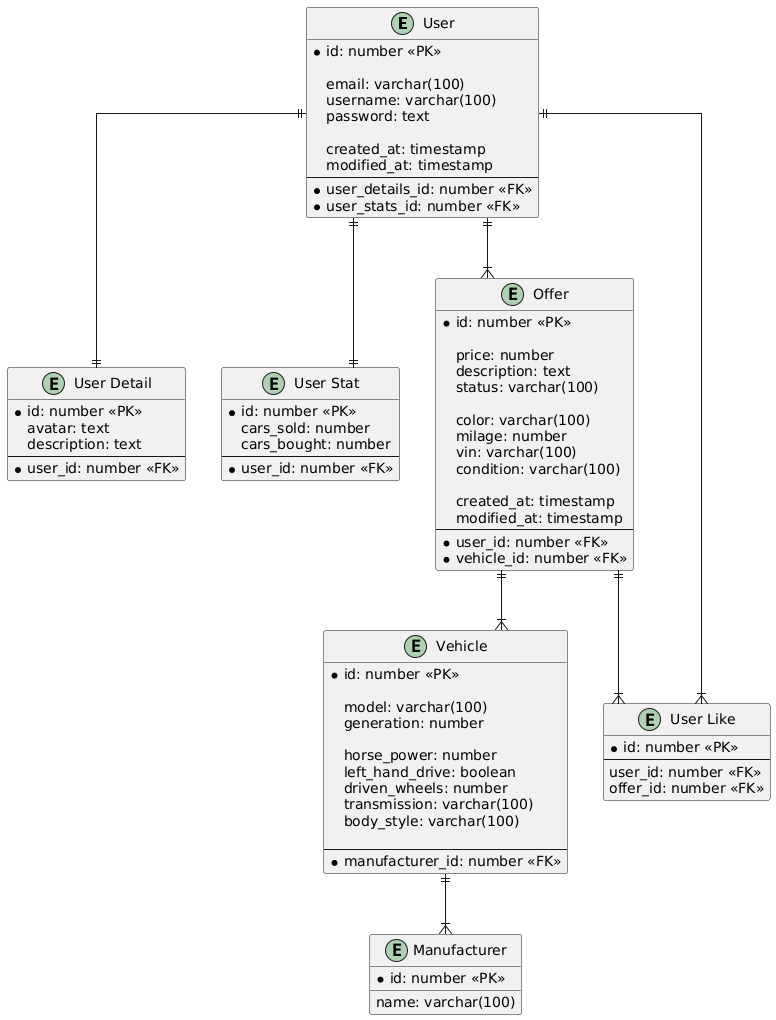
\includegraphics[width=\textwidth]{database.png}

\pagebreak
\part{Baza NoSQL}

\end{document}
